% 先に挿入用の小テストを作成：platex -interaction=nonstopmode -halt-on-error smalltest2_review.tex
% 続いて PDF に変換：dvipdfmx smalltest2_review.dvi
% このフォルダーで2回実行：pdflatex -interaction=nonstopmode -halt-on-error resume3An26w.tex
\documentclass[a4paper,10pt,pdflatex,ja=standard,jafont=ipaex-type1,
  magstyle=real,scale=1]{bxjsarticle}
\usepackage{lmodern}
\usepackage{amsmath,amssymb,mathtools}
\usepackage{geometry}
\geometry{reset,left=22mm,right=22mm,top=20mm,bottom=17mm,
  headheight=13pt,headsep=6mm,footskip=10mm}
\usepackage{xcolor}
\usepackage{enumitem}
\usepackage{array,booktabs,tabularx}
\usepackage{fancyhdr}
\usepackage{lastpage}
\usepackage{pdfpages}
\usepackage{tikz}
\usetikzlibrary{arrows.meta,decorations.pathreplacing}

\definecolor{ink}{HTML}{193A5C}
\definecolor{accent}{HTML}{237D82}
\definecolor{soft}{HTML}{EAF3F3}
\definecolor{muted}{HTML}{52616B}
\newcommand{\coursename}{解析学 II}
\newcommand{\handoutnumber}{3}
\pagestyle{fancy}
\fancyhf{}
\fancyhead[L]{\small\color{ink}\coursename{}・授業要約と演習}
\fancyhead[R]{\small\color{ink}第\handoutnumber 回}
\fancyfoot[C]{\small\color{ink}\thepage/\pageref{LastPage}}
\renewcommand{\headrulewidth}{0.3pt}
\setlength{\parindent}{0pt}
\setlength{\parskip}{2pt}
\setlength{\abovedisplayskip}{5pt}
\setlength{\belowdisplayskip}{5pt}
\setlength{\abovedisplayshortskip}{3pt}
\setlength{\belowdisplayshortskip}{4pt}
\setlist[itemize]{leftmargin=1.8em,itemsep=1pt,topsep=2pt,parsep=0pt}

\newcommand{\handouttitle}[1]{%
  \begin{center}
    {\Large\color{ink}#1}\par\vspace{3mm}
    {\color{accent}\rule{0.88\linewidth}{0.7pt}}
  \end{center}\vspace{-2mm}}
\newcommand{\handout}[2]{%
  \renewcommand{\handoutnumber}{#1}%
  \handouttitle{第#1回\quad #2}}
\newcommand{\topic}[1]{\par\vspace{5pt}%
  {\large\sffamily\mdseries\color{accent}#1}\par\vspace{2pt}}
\newcommand{\keybox}[1]{\par\vspace{3pt}\begingroup
  \setlength{\fboxsep}{4pt}%
  \colorbox{soft}{\parbox{\dimexpr\linewidth-2\fboxsep\relax}{\small #1}}%
  \endgroup\par\vspace{2pt}}
\newenvironment{problems}
  {\begin{enumerate}[leftmargin=2em,itemsep=3pt,topsep=3pt,parsep=0pt,
    font=\color{accent}]}
  {\end{enumerate}}


\newcommand{\examplelabel}[1]{{\sffamily\mdseries\color{ink}#1}}
\newcommand{\problemspace}{\par\vspace{5mm}}
\newcommand{\exercises}{%
  {\color{accent}\hrule height 0.7pt}\vspace{3pt}%
  \topic{演習問題（6題）}%
  {\small 高さは各小長方形の左下の点 $(x_i,y_j)$ で決め、区分求積法で計算しよう。}\par}


% Review Q&A can also be used for actual student feedback when it is available.
\newcommand{\feedback}[2]{%
  \par\addvspace{5pt}\noindent\begin{minipage}{\linewidth}%
  {\color{ink}Q. #1}\par\vspace{1pt}%
  {\color{accent}A. }#2%
  \end{minipage}\par}
\fancypagestyle{smalltestpages}{%
  \fancyhf{}%
  \fancyhead[L]{\small\color{ink}\coursename{}・小テスト}%
  \fancyhead[R]{\small\color{ink}第2回}%
  \fancyfoot[C]{\small\color{ink}\thepage/\pageref{LastPage}}%
  \renewcommand{\headrulewidth}{0.3pt}}

\begin{document}
\fontsize{10pt}{13.5pt}\selectfont
\setlength{\abovedisplayskip}{4pt}
\setlength{\belowdisplayskip}{4pt}
\fancyhead[L]{\small\color{ink}\coursename{}・フィードバック}
\handout{3}{前回のコメントへのフィードバック}
\topic{積分・関数について}

\feedback{中島が一番好きな公式}{%
ガウスが発見した $\displaystyle\sqrt{\pi}=\int_{\mathbb R}e^{-x^2}\,dx$ というのは、個人的に好きな公式です。
ガウスの証明が独創的で、一変数の積分をあえて二変数で積分してから、元に戻すということをしています。
（たぶん第6回くらいにやります。）遠回りすることは、実はよいこともあることを暗示している気がしています。
}

\feedback{有理関数という言葉を初めて聞いた。}{%
分数のことを有理数と呼ぶ関係で、関数の分数を有理関数と呼んだりしますね。
}

\feedback{逆三角関数の微分で有理関数が出るのは不思議。}{%
私も実は不思議です。なんでなんでしょうかね？
}

\feedback{部分分数分解を考えるとうまくいくのが不思議。特異点に分解していくノリかな？}{%
その理解は正しくて、極（分母がゼロになるところ）で分解しているイメージですね。
実は行列の対角化と深い関わりがあります。興味があればぜひ調べてみてください。
}

\feedback{分母の関数に $\sqrt{\cdots}$ が出たとき。}{%
授業では扱っていないですが、$1/\sqrt{1-x^2}$ のときは、$\operatorname{Sin}^{-1}x$ などを使えばよいです。
$1/\sqrt{ax^2+bx+c}$ など、もっと一般の場合は、うまく平方完成と変数変換を用いて
$1/\sqrt{1\pm x^2}$ の形に持っていき、$x=\sin\theta$ や $x=\tan\theta$ などの変数変換をして求めていきます。
その際、積分区間の変化に注意しなければなりません。例を2つ挙げます。

\examplelabel{例：$\displaystyle\int_0^1\frac{dx}{\sqrt{3+2x-x^2}}$。}
$3+2x-x^2=4-(x-1)^2$ と平方完成し、$u=(x-1)/2=\sin\theta$ と置きます。
$x:0\to1$ に対して、$u:-1/2\to0$、$\theta:-\pi/6\to0$ です。
$$
 \int_0^1\frac{dx}{\sqrt{3+2x-x^2}}
 =\int_{-1/2}^0\frac{du}{\sqrt{1-u^2}}
 =\int_{-\pi/6}^0d\theta=\frac{\pi}{6}.
$$
\examplelabel{例：$\displaystyle\int_0^1\frac{dx}{\sqrt{x^2+2x+2}}$。}
$x^2+2x+2=(x+1)^2+1$ と平方完成し、$u=x+1=\tan\theta$ と置きます。
$x:0\to1$ に対して、$u:1\to2$、$\theta:\pi/4\to\operatorname{Tan}^{-1}2$ です。
この区間では $\cos\theta>0$ なので、
$$
 \begin{aligned}
 \int_0^1\frac{dx}{\sqrt{x^2+2x+2}}
 &=\int_1^2\frac{du}{\sqrt{1+u^2}}
 =\int_{\pi/4}^{\operatorname{Tan}^{-1}2}\frac{d\theta}{\cos\theta}\\
 &=\left[\log\left(\frac1{\cos\theta}+\tan\theta\right)\right]_{\pi/4}^{\operatorname{Tan}^{-1}2}
 =\log\frac{2+\sqrt5}{1+\sqrt2}.
 \end{aligned}
$$
}

\feedback{定積分に直して変数変換するとき、積分区間の下の定数は何でもよいか？}{%
これはよい質問で、何でもよいです。結局、定数 $C$ に押し付けてしまうので。
気になるようであれば、具体的に $0$ とかを置くのではなく、定数 $a$ とかを使ってやったりします。
}

\feedback{$t=\tan\theta$ としても同じ答えになるか。}{%
同じ答えになります！この場合は変数変換の際、積分区間で $\operatorname{Tan}^{-1}$ が出てきます。
}

\newpage
\handouttitle{第3回\quad フィードバック（つづき）}

\topic{小テスト・学習の進め方について}

\feedback{3)が合っているか不安。}{%
合っています（導出も正しいです）が、積分区間をちゃんと書いたほうがよいかなと思います。
}

\feedback{教科書の一般化したものを理解したほうがよいか？}{%
したほうがよいと思いますが、必ずしも覚える必要はないです。
むしろ公式を覚えるよりやり方を覚えたほうが有益ですし、忘れにくいです。
}

\feedback{付属組と受験組で、積分は力の差が出やすい。}{%
面白い話ですね。でも積分計算は努力に比例して伸びる分野だと思います。
}

\topic{授業の予定・レジュメについて}

\feedback{中間の範囲。}{%
第7回までの範囲です。広義積分あたりまででしょうか？
}

\feedback{レジュメの題名が解析学IIになっている。}{%
大学数学では微積分を解析学と呼ぶことが多いので、こういう名前を付けてしまいました。特に意味はないです。
}

\feedback{レジュメのアップロードが速くて助かる。}{%
これからも頑張りますね。
}

\topic{日常のこと}

\feedback{夏休み気分が抜けない}{%
もう3週間たっていますよ！
}

\feedback{中島も1限はつらいか。}{%
もちろんつらいです。南武線が限界状態ですので。
}

\feedback{3日連続1限だるい。}{%
言葉遣い！！
}

\feedback{バイトを始めて週2になると言われてシフトを組んだら、週4になった。}{%
あら。
}

\feedback{タブレットが壊れた。}{%
頑張って復旧してください。
}

\feedback{数学の問題を解いていると、腰や肩が痛くなる。}{%
やり続けると、そんなに悪くないですよ。
}

\feedback{冬が寂しいです。}{%
もうすぐ来ますから待ちましょう。
}

\feedback{ヨーグルトにはキウイと蜂蜜がよい。}{%
キウイは試したことがないですね。手に入りづらいのですかね。
}
\clearpage

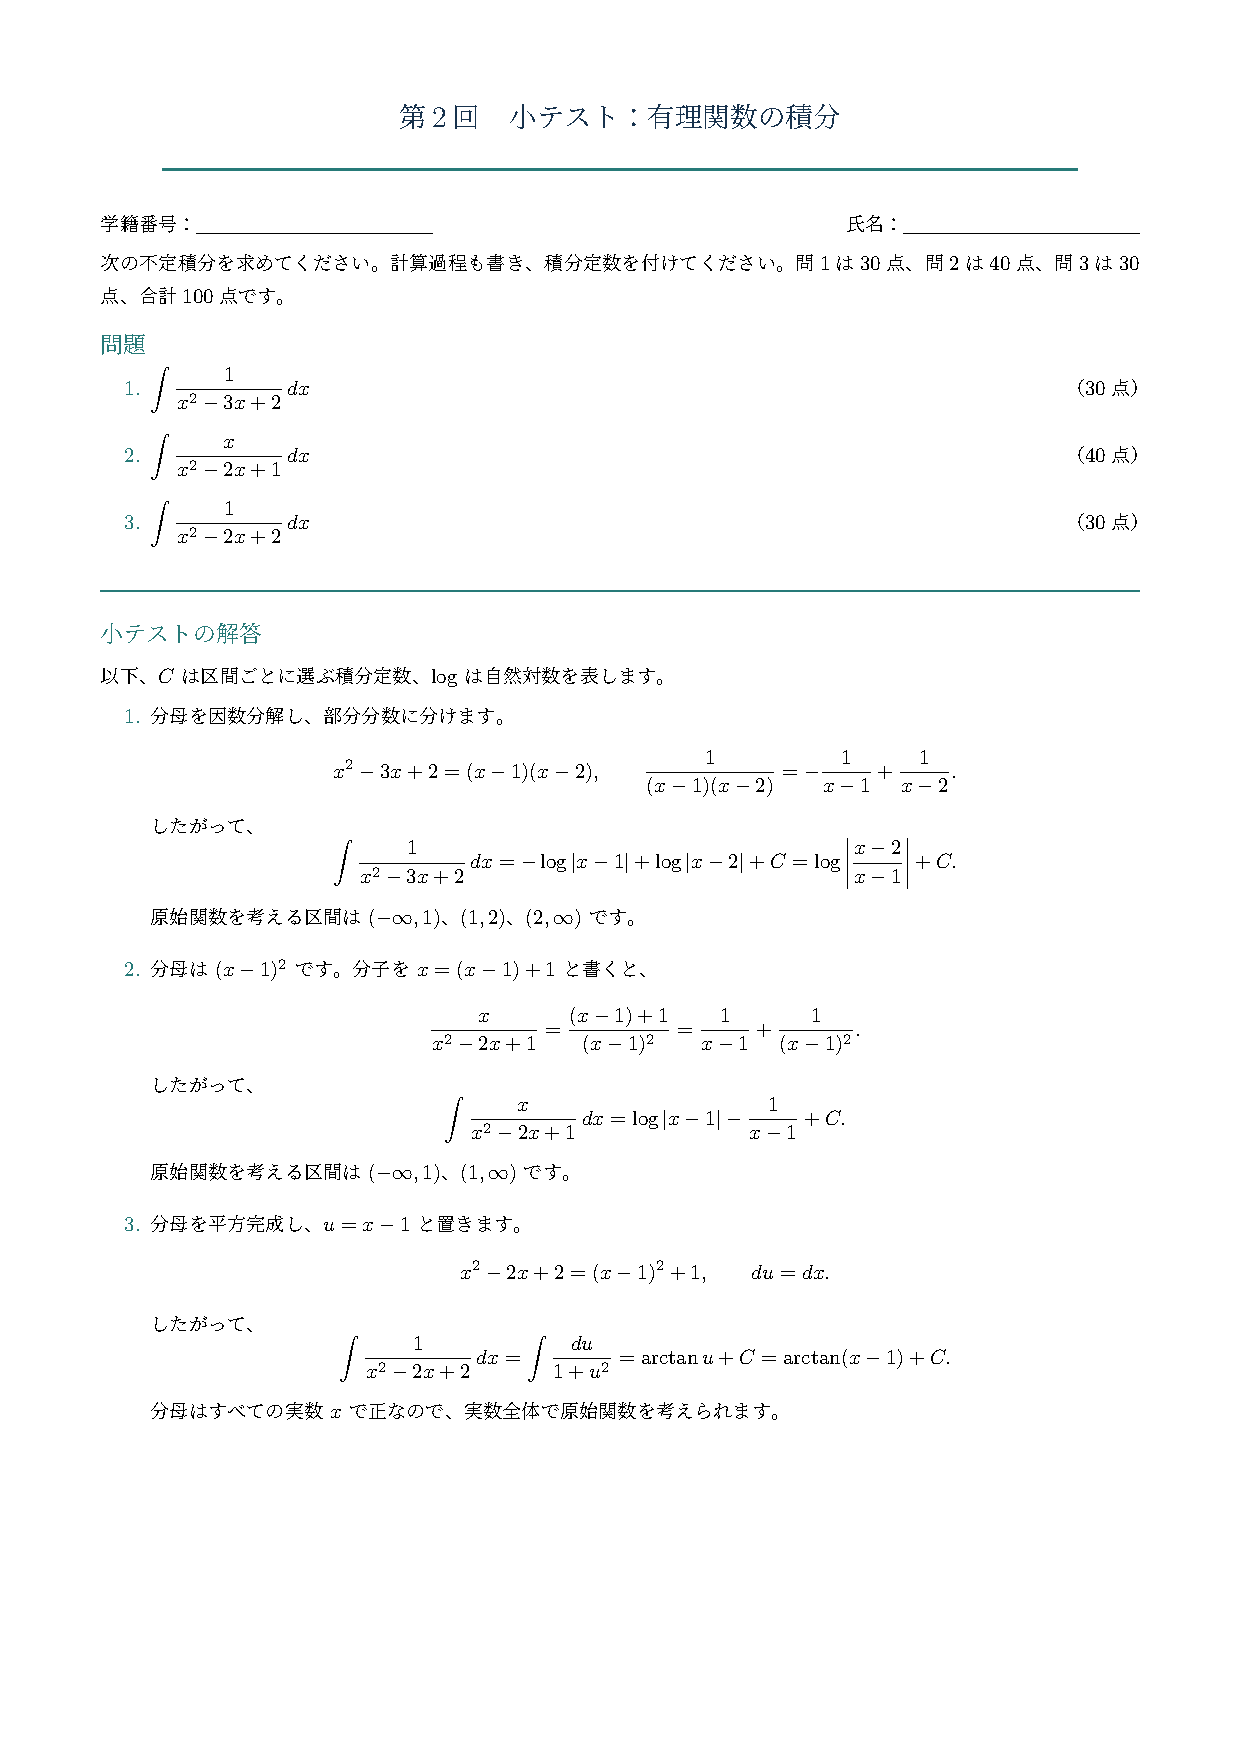
\includepdf[pages=-,pagecommand={\thispagestyle{smalltestpages}}]{smalltest2_review.pdf}

\fancyhead[L]{\small\color{ink}\coursename{}・授業要約と演習}
\fancyhead[R]{\small\color{ink}第\handoutnumber 回}
\handout{3}{重積分の定義}\label{lesson-start}
\keybox{到達目標：長方形を $N\times M$ 個に分け、左下の点 $(x_i,y_j)$ で決めた高さの柱の体積を足し、
$N,M\to\infty$ の極限として重積分を理解する。}

\topic{復習：一次元の区分求積法}
連続関数 $g$ を区間 $[a,b]$（$a<b$）で考える。
$n$ 等分した幅を $\Delta=(b-a)/n$ とすると、各小区間の左端は $a+(i-1)\Delta$（$i=1,\ldots,n$）なので
$$
 \int_a^b g(t)\,dt
 =\lim_{n\to\infty}\sum_{i=1}^n g\bigl(a+(i-1)\Delta\bigr)\,\Delta.
$$
一次元では「高さ $\times$ 幅」の和で面積を求め、
二次元では「高さ $\times$ 底面積」の和で体積を求める。

\examplelabel{例：$g(t)=t$、$[a,b]=[0,1]$。}
$$
 \sum_{i=1}^n\frac{i-1}{n}\cdot\frac1n
 =\frac1{n^2}\cdot\frac{n(n-1)}2
 =\frac{n-1}{2n}\longrightarrow\frac12
 =\int_0^1 t\,dt.
$$
\keybox{計算に使う公式：
$\displaystyle\sum_{i=1}^n(i-1)=\frac{n(n-1)}2$、\quad
$\displaystyle\sum_{i=1}^n(i-1)^2=\frac{n(n-1)(2n-1)}6$。}

\topic{長方形を $N\times M$ 個に分ける}
$K=[a,b]\times[c,d]$（$a<b$、$c<d$）上の有界な実数値関数 $f(x,y)$ を考える。
$x$ 方向を $N$ 等分、$y$ 方向を $M$ 等分する（$N,M$ は正の整数）。
$$
 \Delta_x=\frac{b-a}{N},\quad \Delta_y=\frac{d-c}{M},\qquad
 x_i=a+(i-1)\Delta_x,\quad y_j=c+(j-1)\Delta_y.
$$
$x_1=a,x_{N+1}=b$、$y_1=c,y_{M+1}=d$ であり、$i=1,\ldots,N$、$j=1,\ldots,M$ に対し、小長方形を
$Q_{ij}=[x_i,x_{i+1}]\times[y_j,y_{j+1}]$ とする。
面積は $\Delta_x\Delta_y$ であり、高さはすべて左下の点 $(x_i,y_j)$ で決める。

\begin{center}
\begin{minipage}[b]{0.48\linewidth}
\centering
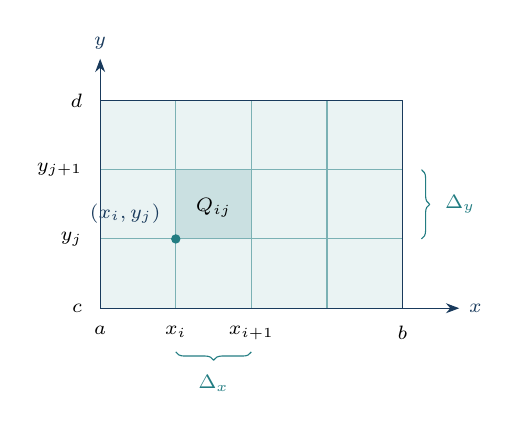
\begin{tikzpicture}[x=0.96cm,y=0.88cm,>=Stealth,
  every node/.style={font=\scriptsize},line join=round]
 \fill[soft] (0,0) rectangle (4,3);
 \fill[accent!24] (1,1) rectangle (2,2);
 \draw[accent!60,thin,step=1] (0,0) grid (4,3);
 \draw[ink] (0,0) rectangle (4,3);
 \draw[->,ink] (0,0) -- (4.75,0) node[right] {$x$};
 \draw[->,ink] (0,0) -- (0,3.6) node[above] {$y$};
 \node[below=3pt] at (0,0) {$a$};
 \node[below=3pt] at (4,0) {$b$};
 \node[left=3pt] at (0,0) {$c$};
 \node[left=3pt] at (0,3) {$d$};
 \node[below=3pt] at (1,0) {$x_i$};
 \node[below=3pt] at (2,0) {$x_{i+1}$};
 \node[left=3pt] at (0,1) {$y_j$};
 \node[left=3pt] at (0,2) {$y_{j+1}$};
 \node at (1.5,1.45) {$Q_{ij}$};
 \fill[accent] (1,1) circle (1.7pt);
 \node[above left=2pt,text=ink] at (1,1) {$(x_i,y_j)$};
 \draw[decorate,decoration={brace,mirror,amplitude=3pt},accent]
   (1,-0.63) -- (2,-0.63) node[midway,below=5pt] {$\Delta_x$};
 \draw[decorate,decoration={brace,mirror,amplitude=3pt},accent]
   (4.25,1) -- (4.25,2) node[midway,right=5pt] {$\Delta_y$};
\end{tikzpicture}\par
{\small (a) 平面の分割（図は $N=4$、$M=3$）}
\end{minipage}\hfill
\begin{minipage}[b]{0.49\linewidth}
\centering
\begin{tikzpicture}[x={(0.95cm,-0.16cm)},y={(0.40cm,0.35cm)},
 z={(0cm,0.88cm)},>=Stealth,every node/.style={font=\scriptsize},
 line join=round]
 \draw[->,ink] (0,0,0) -- (4.8,0,0) node[right] {$x$};
 \draw[->,ink] (0,0,0) -- (0,0,4.1) node[above] {$z$};
 \foreach \j in {3,2,1}{
  \foreach \i in {1,2,3,4}{
   \pgfmathsetmacro{\h}{0.8+0.34*\i+0.23*\j}
   \filldraw[fill=accent!24,draw=accent!80,thin]
    (\i-1,\j-1,0) -- (\i,\j-1,0) -- (\i,\j-1,\h)
     -- (\i-1,\j-1,\h) -- cycle;
   \filldraw[fill=accent!43,draw=accent!80,thin]
    (\i,\j-1,0) -- (\i,\j,0) -- (\i,\j,\h)
     -- (\i,\j-1,\h) -- cycle;
   \filldraw[fill=soft,draw=accent!80,thin]
    (\i-1,\j-1,\h) -- (\i,\j-1,\h) -- (\i,\j,\h)
     -- (\i-1,\j,\h) -- cycle;
  }
 }
 % Indicate the y direction at the exposed edge of the base.
 \draw[->,ink] (4,3,0) -- (4,4.2,0) node[above right] {$y$};
 \draw[ink,thin] (3.5,0.5,2.39) -- (4.8,0.4,4.3)
   node[above left] {高さ $f(x_i,y_j)$};
 \node[below=6pt,text=ink] at (2,0,0) {底面積 $\Delta_x\Delta_y$};
\end{tikzpicture}\par
{\small (b) 小長方形の上に柱を立てる（$f\ge0$）}
\end{minipage}
\end{center}
\vspace{-2mm}

\topic{小さな柱の体積を足す}
柱1本の体積は「高さ $\times$ 底面積」なので、その和（リーマン和）は
$$
 S_{N,M}(f)=\sum_{i=1}^N\sum_{j=1}^M f(x_i,y_j)\,\Delta_x\Delta_y.
$$

\newpage
% 授業要約の2ページ目の上半分に、残りの説明と例題を置く。
\noindent\begin{minipage}[b][\dimexpr0.5\textheight-\parskip\relax][t]{\linewidth}
\topic{左下の点で作った和の極限}
\keybox{$K$ 上の連続関数 $f$ について、各小長方形の左下の点 $(x_i,y_j)$ で高さを決める。
$N,M$ をともに限りなく大きくしたときの和の極限を、$K$ 上の $f$ の重積分と呼ぶ。
$$
 \iint_K f(x,y)\,dx\,dy
 :=\lim_{\substack{N\to\infty\\M\to\infty}}
 \sum_{i=1}^N\sum_{j=1}^M f(x_i,y_j)\,\Delta_x\Delta_y.
$$
}
連続関数ではこの極限が存在する。$N,M$ はそれぞれ独立に大きくする。

\examplelabel{例：$K=[0,1]^2$、$f(x,y)=xy$。}
$\Delta_x=1/N$、$\Delta_y=1/M$、$(x_i,y_j)=((i-1)/N,(j-1)/M)$ より
$$
 S_{N,M}(f)=\frac1{N^2M^2}
 \left(\sum_{i=1}^N(i-1)\right)\left(\sum_{j=1}^M(j-1)\right)
 =\frac{(N-1)(M-1)}{4NM}\longrightarrow\frac14.
$$
したがって $\displaystyle\iint_{[0,1]^2}xy\,dx\,dy=\frac14$ である。

\topic{一般の領域では、外側の高さを0にする}
三角形や円盤などの有界な領域 $D\subset\mathbb R^2$ 上の、有界な連続関数 $f$ を考える。
$D$ を含む長方形 $K$ を取り、$D$ の外側で高さを0にした関数を使う。
$$
 \widetilde f(x,y)=\begin{cases}
  f(x,y),&(x,y)\in D,\\
  0,&(x,y)\in K\setminus D.
 \end{cases}
 \qquad
 \iint_D f(x,y)\,dx\,dy:=\iint_K\widetilde f(x,y)\,dx\,dy.
$$
右辺は、左下の点 $(x_i,y_j)$ における $\widetilde f$ の値で作った和の極限で計算する。
三角形や円などでは、高さ1の積分 $\displaystyle\iint_D1\,dx\,dy$ は領域の面積になる。

\end{minipage}\par\nointerlineskip
% 授業要約の2ページ目の下半分に、演習問題と書き込み用の余白を置く。
\noindent\begin{minipage}[b][0.5\textheight][t]{\linewidth}
\exercises
\begin{problems}
\item 一次元の区分求積法を用い、$[0,1]$ を $n$ 等分した左端の和から
$\displaystyle\int_0^1 t^2\,dt$ を求めよ。\problemspace

\item $K=[0,2]\times[0,3]$ を $N=2,M=3$ 等分するとき、
小長方形の面積と、$f\equiv4$ のリーマン和を求めよ。\problemspace

\item $K=[0,1]^2$、$f(x,y)=x+y$ とする。
$N\times M$ 分割のリーマン和と、$N,M\to\infty$ の極限を求めよ。\problemspace

\item $K=[0,1]^2$、$f(x,y)=xy$ の $2\times2$ 分割のリーマン和を求め、
重積分の値 $1/4$ と比較せよ。\problemspace

\item $K=[0,2]\times[0,1]$、$f(x,y)=x^2y$ とする。
$N\times M$ 分割のリーマン和を計算し、重積分の値を求めよ。\problemspace


\item $D=\{(x,y):0\le y\le x\le1\}$ とする。
$\iint_D1\,dx\,dy$ を、図形の面積と $[0,1]^2$ 上の区分求積法の両方で求めよ。\problemspace

\end{problems}
\end{minipage}

\newpage
\handouttitle{第3回\quad 演習問題の解答}
{\small 各小長方形の左下の点 $(x_i,y_j)$ で高さを決め、幅と面積を確かめながら計算しよう。}\par
\begin{problems}
\setlength{\itemsep}{7pt}
\item 幅は $1/n$、左端は $(i-1)/n$（$i=1,\ldots,n$）だから
$$
 \int_0^1t^2\,dt
 =\lim_{n\to\infty}\frac1{n^3}\sum_{i=1}^n(i-1)^2
 =\lim_{n\to\infty}\frac{n(n-1)(2n-1)}{6n^3}=\frac13.
$$

\item $\Delta_x=2/2=1$、$\Delta_y=3/3=1$ より、小長方形の面積は1。
小長方形は6個、すべて高さ4なので
$$
 S_{2,3}(f)=\sum_{i=1}^2\sum_{j=1}^3 4\cdot1=24.
$$
これは底面積6、高さ4の直方体の体積と一致する。

\item $(x_i,y_j)=((i-1)/N,(j-1)/M)$、$\Delta_x\Delta_y=1/(NM)$ より
$$
 \begin{aligned}
 S_{N,M}(f)
 &=\frac1{NM}\sum_{i=1}^N\sum_{j=1}^M\left(\frac{i-1}{N}+\frac{j-1}{M}\right)\\
 &=\frac1{N^2}\sum_{i=1}^N(i-1)+\frac1{M^2}\sum_{j=1}^M(j-1)
 =\frac{N-1}{2N}+\frac{M-1}{2M}\longrightarrow1.
 \end{aligned}
$$
$x$ だけの項は $j$ について $M$ 回、$y$ だけの項は $i$ について $N$ 回現れる。

\item 左下の点は $(0,0),(1/2,0),(0,1/2),(1/2,1/2)$、底面積は各 $1/4$ なので
$$
 S_{2,2}(f)=\frac14\left(0+0+0+\frac14\right)=\frac1{16}.
$$
重積分の値 $1/4$ より $3/16$ 小さい。左下の点では $xy$ が各小長方形内の最小値となるためである。

\item $\Delta_x=2/N$、$\Delta_y=1/M$、$(x_i,y_j)=(2(i-1)/N,(j-1)/M)$ として
$$
 \begin{aligned}
 S_{N,M}(f)
 &=\frac8{N^3M^2}
   \left(\sum_{i=1}^N(i-1)^2\right)\left(\sum_{j=1}^M(j-1)\right)\\
 &=\frac23\left(1-\frac1N\right)\left(2-\frac1N\right)
   \left(1-\frac1M\right)\longrightarrow\frac43.
 \end{aligned}
$$
よって $\iint_{[0,2]\times[0,1]}x^2y\,dx\,dy=4/3$ である。

\item $D$ は底辺・高さがともに1の直角三角形なので、面積は $1/2$。
$[0,1]^2$ を $N\times M$ 個に分け、左下の点 $(x_i,y_j)=((i-1)/N,(j-1)/M)$ で高さを決める。
$D$ の外で高さを0にした関数 $\widetilde f$ の値は、$(j-1)/M\le(i-1)/N$ なら1、それ以外では0である。
各 $i=1,\ldots,N$ について $(j-1)/M\le(i-1)/N$ を満たす $j\in\{1,\ldots,M\}$ の個数を $k_i$ とおくと、
$$
 \frac{M(i-1)}{N}<k_i\le\frac{M(i-1)}{N}+1,\qquad
 S_{N,M}(\widetilde f)=\frac1{NM}\sum_{i=1}^N k_i.
$$
したがって、
$$
 \frac{N-1}{2N}
 <S_{N,M}(\widetilde f)\le\frac{N-1}{2N}+\frac1M.
$$
$N,M\to\infty$ のとき両端は $1/2$ に近づくので、
$$
 \iint_D1\,dx\,dy
 =\lim_{\substack{N\to\infty\\M\to\infty}}S_{N,M}(\widetilde f)
 =\frac12.
$$
図形の面積と一致する。
\end{problems}
\end{document}
